\section{Metodologia}

O repositório sbc-template utiliza das mais variadas tecnologias do github para a automação de todo o processo, dentre elas as principais está a Devcontainer e a Actions.

\subsection{Devcontainer}
Os containers docker são soluções de virtualização semelhantes às máquinas virtuais, porém mais enxutas e apenas com as informações necessárias para a sua execução~\cite{vitalino:01}. Para a criação de um container utilizamos uma imagem Docker, uma espécie de documento que declara as informações necessárias para determinado container. Entre essas informações podemos citar por exemplo o sistema operacional, aplicativos que o container deve conter, comandos iniciais ao criar o container e conexões de rede local.
Os devcontainers ou containers de desenvolvimento são containers docker que possuem um embiente completo com todas as configurações necessárias para o desenvolvimento de uma aplicação~\cite{github:01}. No repositório SBC template usamos o devcontainer para configurar todo o projeto latex, com o compilador para o pdf, ferramentas de edição e formatação do arquivo e uso de extensões do Visual Studio Code. Assim além de um projeto completo poder ser usado em uma maquina física com uma configuração automática, o mesmo pode ser facilmente removido sem muitas complicações em desisntalar o projeto e suas dependências.
Na figura~\ref{fig:image12}, podemos visualizar o projeto sbc-template em execução no Visual Studio Code e ao lado o container em execução no docker. Podemos analisar o uso da CPU e memória do container em tempo real.

\begin{figure}[ht]
	\centering
	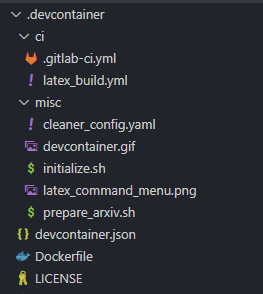
\includegraphics[width=.5\textwidth]{./images/image12.png}
	\caption{Visualizando o devcontainer pelo Visual Studio Code e dashboard do Docker}
	\label{fig:image12}
\end{figure}
A implantação do devcontainer consistiu nos diretórios .devcontainer e .vscode, que respectivamente possui uma serie de arquivos de configuração para instalação de dependências e scripts para a execução dessas dependências no container; e arquivos de configuração para o comportamento das dependências.
No diretório .devcontainer temos o arquivo devcontainer.json que declara a imagem Docker pelo arquivo Dockerfile, a lista de extensões desejáveis e o script de inicialização do devcontainer. O dockerfile possui uma imagem de referencia  danteev/texlive que cria um container ubuntu com o compilador TexLive. O script initialize.sh inicia a configuração do Visual Studio Code e o CI (continuous integration) do container. As configurações de CI permitem que todas as vezes que o projeto é alterado, um novo arquivo PDF é gerado e sobrescreve o antigo na pasta article.

\subsection{Actions}
O Github Actions 

O Github Actions é uma plataforma criada pelo GitHub que utiliza de containers docker para a realização de integração contínua e entrega cotínua (CI/CD)~\cite{github:02}. Através do GitHub Actions podemos criar testes automatizados, validações de projeto, criar versões compiladas de arquivos, entre outras atividades~\cite{github:02}. Em nosso projeto utilizamos o Github Actions para duas atividades, em ambos os casos para gerar um pdf final do projeto. O que diferencia em cada caso é que temos na pasta .github, o arquivo $latex\_build.yml$ que gera um PDF em branchs de pull requests abertas, ao subir um novo commit, o pdf é gerado e em seguida é criado um comentário na pull request. Ja o arquivo $latex\_release.yml$ configura o PDF para virar uma versão de release na página inicial do repositório.

A vantagem do github actions é permitir a edição e atualização do projeto sem necessáriamente criar um ambiente devcontainer para edições rápidas e discussões entre autor e orientador. Ao alterar qualquer arquivo no site do github, as actions se encarregam de gerar um novo artigo final em PDF.